\section{Introduction}

An experimental program focused on the search for exotics and the study of rare mesons requires measurements
of a broad range of final states in order to consolidate the possible evidence for their production by looking at different
decay modes and exploring poorly studied reaction channels~\cite{mesonex}. The characteristics of the detector
and the trigger conditions foreseen for the experiment - 11~GeV electron beam scattering on a 5-cm-long LH$_2$
target with multiple particles in the final state - will allow  measurements of many final states simultaneously. While
the hadrons will be detected in the CLAS12 spectrometer~\cite{overview}, the electron scattered at very small
angles (2.5$^\circ$ to 4.5$^\circ$ in polar angle) and low four-momentum transfer, $Q^2$,  will be detected in the
Forward Tagger (FT), i.e. in the kinematics of quasi-real photoproduction. The FT  specifications were thus defined
to have optimal electron detection at low angles, compatible with the high rate of electromagnetic background. To
reconstruct the  quasi-real photon variables, it is necessary to measure the scattered electron three momentum.
The relevant quantities are:

\begin{itemize}
\item the energy $E_{e'}$: since the photon energy is given by $E_\gamma =\nu=E_{beam}-E_{e'}$ and its linear
  polarization by $P_\gamma=\epsilon\sim\left( 1+\frac{\nu^2}{2 E_{beam} E_{e'}}\right)^{-1}$,
\item the azimuthal angle $\phi_{e'}$ to determine the polarization plane, 
\item the polar angle angle $\theta_{e'}$: since $Q^2 = 4 E_{beam} E_{e'} \sin^2{\theta_{e'}/2}$.
\end{itemize}

The FT is composed of: an electromagnetic calorimeter  (FT-Cal) to identify the electron by measuring its
electromagnetic shower energy and to provide a fast trigger signal, a Micromegas tracker (FT-Trk) to measure
the scattering angles ($\theta_{e'}$ and $\phi_{e'}$), and a  scintillation counter (FT-Hodo) to provide $e/\gamma$
separation. The FT-Cal and FT-Hodo also provide fast signals to trigger the data acquisition~\cite{daq} in coincidence
with signals from CLAS12. Fig.~\ref{fig:ftcad} shows a CAD rendering of the FT.

\begin{figure}[th!]
\centering 
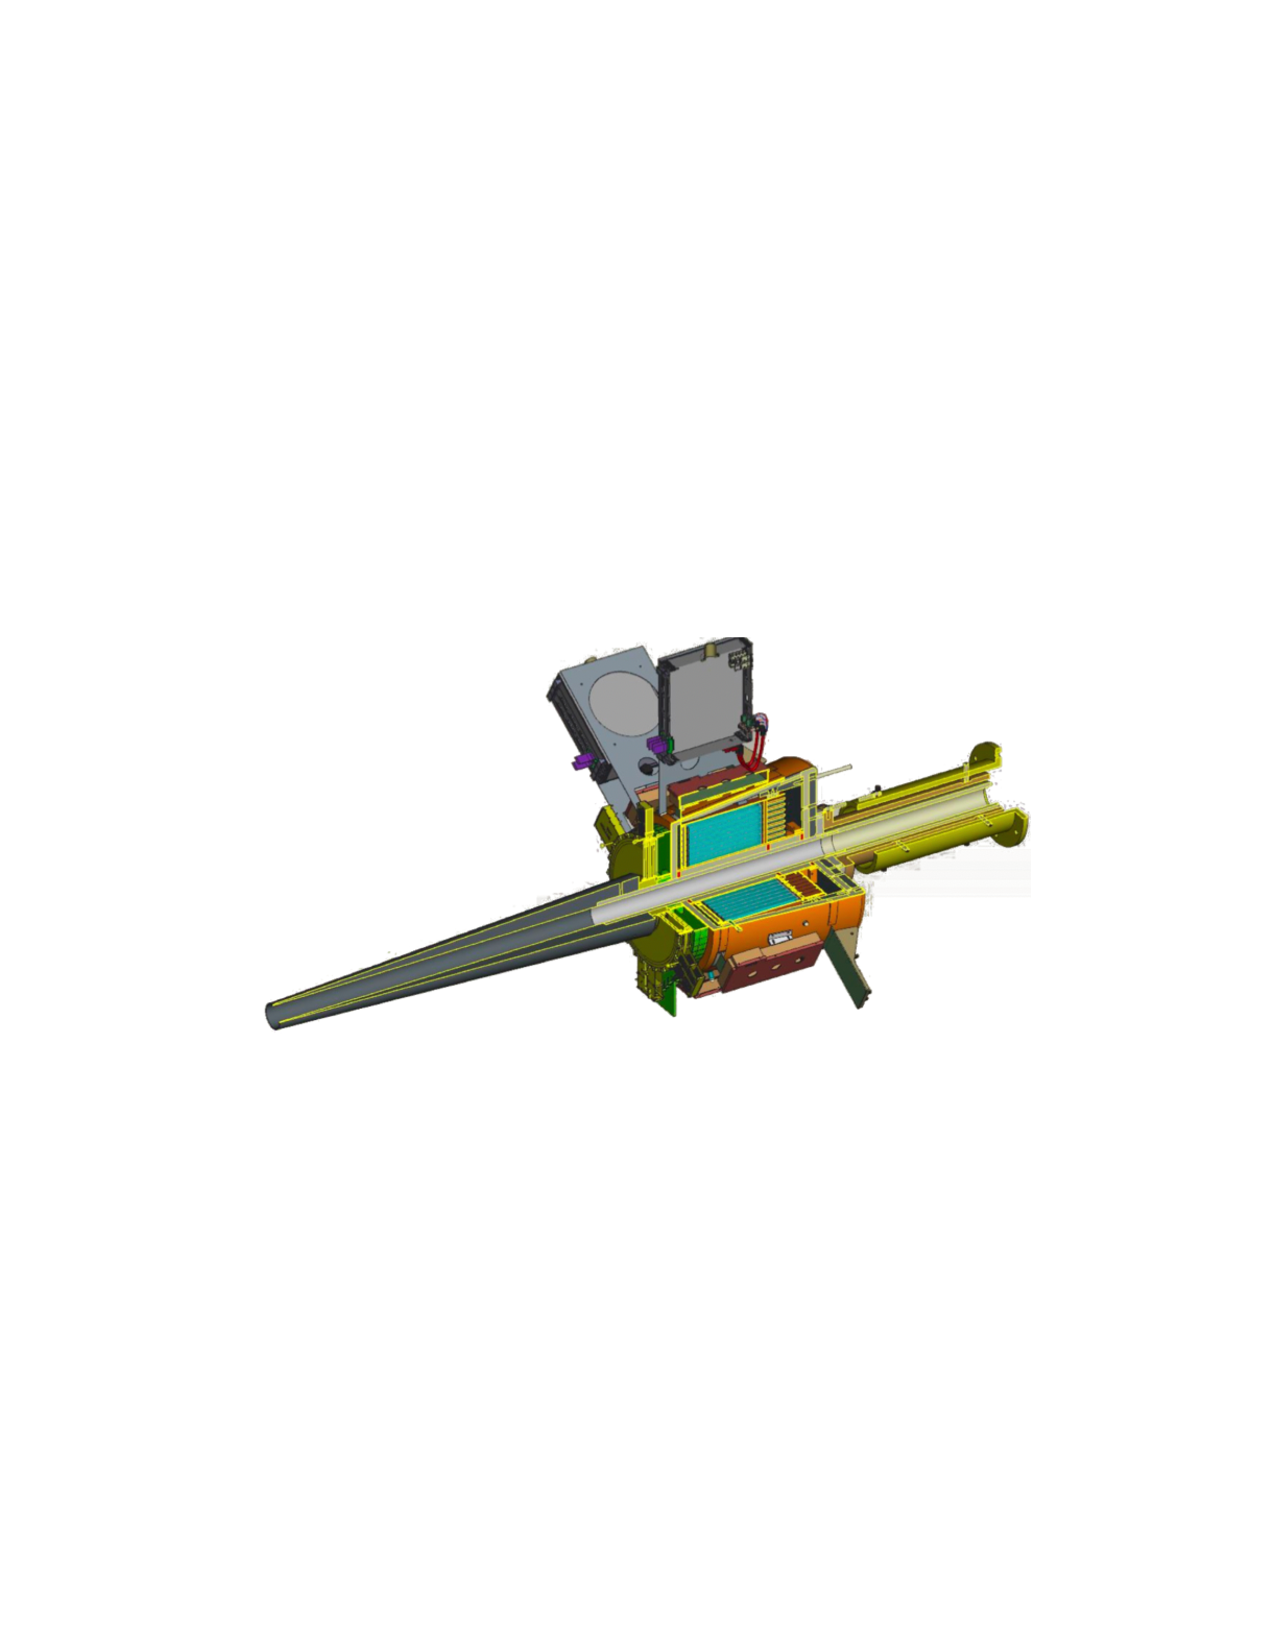
\includegraphics[width=\columnwidth]{./fig/ft-model.pdf} 
\caption{CAD drawing of the Forward Tagger. The FT calorimeter shown in cyan is located at about 185~cm from the
  beam-target interaction point and is enclosed in a copper and Rohacell case to provide thermal insulation. The scintillation
  counter (green) and the tracker (yellow) are located in front of the calorimeter. A tungsten cone (gray) shields the FT
  from M{\o}ller electrons and electromagnetic background created by the beam. } 
\label{fig:ftcad} 
\end{figure}

The calorimeter, the scintillation counter, and the tracker are placed between the High Threshold Cherenkov
Counter (HTCC)~\cite{htcc} and the torus magnet support~\cite{magnets}, at about 185~cm downstream of the
nominal target position. The close proximity to the beamline ($2.5^\circ$ corresponds to $\sim$8~cm radial distance
from the beamline) and the
limited space available (at most $\sim$40~cm along the beam axis), requires a compact calorimeter of small
radiation length and with very good radiation hardness. Figure~\ref{fig:ftinclas12} shows a CAD drawing of the
FT integrated in CLAS12. The FT-Hodo scintillation counter, placed in front of the calorimeter, is made of plastic
scintillator tiles  read-out by silicon photomultipliers via wavelength shifting fibers. The FT-Trk detector is then
located in front of the FT-Hodo to extend the acceptance of the FT down to 2.5$^\circ$. All of these
components were designed to fit within a 5.5$^{\circ}$ cone around the beam axis to have minimal impact on the operation
and acceptance of the CLAS12 equipment in the forward direction.

\begin{figure}[th!]
\centering 
\includegraphics[width=\columnwidth]{./fig/ft_cad.eps} 
\caption{CAD drawing showing the integration of the FT in CLAS12. The FT is located in the free space between
  the High Threshold Cherenkov Counter (HTCC)~\cite{htcc} and the first Drift Chamber (DC) region~\cite{dc}.} 
\label{fig:ftinclas12} 
\end{figure}
